\documentclass{standalone}
\usepackage{tikz}
\usepackage{amsmath}
\usepackage{amssymb}
\usetikzlibrary{decorations}
\usepackage{pgfplots}
\usepgfplotslibrary{groupplots}
\pgfplotsset{compat=newest}
\usepackage{subcaption}

\usepackage{xcolor}
\definecolor{TUDa-0d}{cmyk/RGB/HTML}{0,0,0,.8/83,83,83/535353}
\definecolor{TUDa-0c}{cmyk/RGB/HTML}{0,0,0,.6/137,137,137/898989}
\definecolor{TUDa-0b}{cmyk/RGB/HTML}{0,0,0,.4/181,181,181/B5B5B5}
\definecolor{TUDa-0a}{cmyk/RGB/HTML}{0,0,0,.2/220,220,220/DCDCDC}
\definecolor{TUDa-10c}{cmyk/RGB/HTML}{.5,1,.3,0/149,17,105/951169}

\definecolor{PoleTip}{named}{magenta}
\definecolor{IronYoke}{named}{violet}
\definecolor{IronYoke Right Middle}{named}{red}
\definecolor{IronYoke Right Lower}{named}{orange}
\definecolor{Air1}{named}{blue}
\definecolor{Air2}{named}{purple}
\definecolor{Air3}{named}{teal}
\definecolor{Current}{named}{yellow}

\definecolor{Dirichlet bnd.}{named}{black}
\definecolor{Neumann bnd.}{named}{green}


\newcommand*{\addheight}[2][.5ex]{%
  \raisebox{0pt}[\dimexpr\height+(#1)\relax]{#2}%
}

\begin{document}
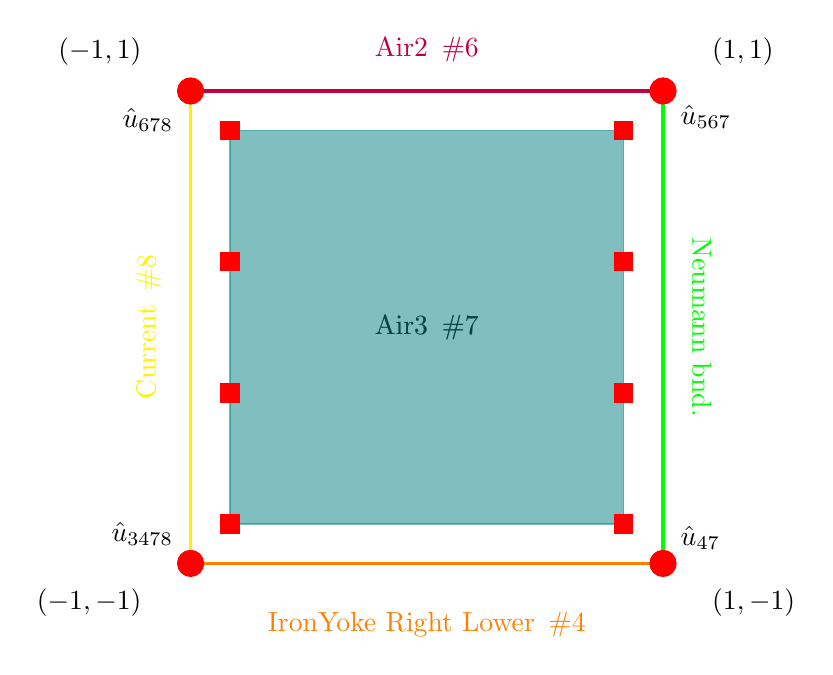
\begin{tikzpicture}
% Domain
\def\dom{Air3}
% Right
\def\rc{Neumann bnd.}
% Left
\def\lc{Current}
% Top
\def\tc{Air2}
% Bottom
\def\bc{IronYoke Right Lower}


\def\r{\textcolor{\rc}{\rc}}
\def\l{\textcolor{\lc}{\lc \, \#8}}
\def\t{\textcolor{\tc}{\tc \, \#6}}
\def\b{\textcolor{\bc}{\bc\, \#4}}
\node[opacity = 0.8] (cr) at (0,0){\dom \, \#7};

\def\r{\textcolor{\rc}{\rc}}
\def\l{\textcolor{\lc}{\lc \, \#8}}
\def\t{\textcolor{\tc}{\tc \, \#6}}
\def\b{\textcolor{\bc}{\bc \, \#4}}


\node[opacity = 0.8] (cr) at (0,0){\dom \, \#7};
\node[anchor=south, rotate = 0] (top) at ( 0, 3.25){\t};
\node[anchor=north] (bottom) at ( 0, -3.5) {\b};
\node[anchor=south, rotate = 90] (left) at ( -3.25, 0){\l};
\node[anchor=south, rotate = -90] (right) at ( 3.25, 0){\r};



\coordinate (xmm) at (-3,-3);
\coordinate (xmm2) at (-2.5,-2.5);

\node[anchor = east] (xmm_l) at (-3.5,-3.5){$(-1,-1)$};

\coordinate (xpm) at ( 3,-3);
\coordinate (xpm2) at ( 2.5,-2.5);

\node[anchor = west] (xpm_l) at (3.5,-3.5){$(1,-1)$};

\coordinate (xpp) at ( 3, 3);
\coordinate (xpp2) at ( 2.5, 2.5);

\node[anchor = west] (xpm_l) at (3.5,3.5){$(1,1)$};

\coordinate (xmp) at (-3,3);
\coordinate (xmp2) at (-2.5,2.5);

\node[anchor = east] (xpm_l) at (-3.5,3.5){$(-1,1)$};

\draw[\bc, very thick] (xmm)--(xpm);
\draw[\rc, very thick] (xpm)--(xpp);
\draw[\tc, very thick] (xpp)--(xmp);
\draw[\lc, very thick] (xmp)--(xmm);


\filldraw[\dom, opacity = 0.5] (xmm2)--(xpm2)--(xpp2)--(xmp2)--(xmm2);





\node[rectangle, draw, red, fill = red] (p1) at (-2.5,-2.5) {};
%\node[rectangle, draw, red, fill = red] (p2) at (-0.8333,-2.5) {};
%\node[rectangle, draw, red, fill = red] (p3) at (0.8333,-2.5) {};

\node[rectangle, draw, red, fill = red] (p2) at (-2.5, -0.8333) {};
\node[rectangle, draw, red, fill = red] (p3) at (-2.5, 0.8333) {};
\node[rectangle, draw, red, fill = red] (p4) at (2.5,-2.5) {};

\node[rectangle, draw, red, fill = red] (p5) at (-2.5,2.5) {};
%\node[rectangle, draw, red, fill = red] (p6) at (-0.8333,2.5) {};
%\node[rectangle, draw, red, fill = red] (p7) at (0.8333,2.5) {};

\node[rectangle, draw, red, fill = red] (p2) at (2.5, -0.8333) {};
\node[rectangle, draw, red, fill = red] (p3) at (2.5, 0.8333) {};
\node[rectangle, draw, red, fill = red] (p8) at (2.5,2.5) {};



\node[anchor = south west] (p10) at (3.1,2.4) {$\hat{u}_{567}$};
\node[anchor = north east] (p11) at (-3.1,2.9) {$\hat{u}_{678}$};
\node[anchor = north west] (p10) at (3.1,-2.4) {$\hat{u}_{47}$};
\node[anchor = south east] (p11) at (-3.1,-2.9) {$\hat{u}_{3478}$};

\node[circle, draw, red, fill = red, opacity = 1] (p9) at (-3,3) {};
\node[circle, draw, red, fill = red, opacity = 1] (p10) at (3,3) {};
\node[circle, draw, red, fill = red, opacity = 1] (p9) at (3,-3) {};
\node[circle, draw, red, fill = red, opacity = 1] (p10) at (-3,-3) {};


\end{tikzpicture}



\end{document}

\begin{comment}
	
% Pole Tip
%--------------------------------------------%
% Domain
\def\dom{PoleTip}
% Right
\def\rc{Current}
% Left
\def\lc{Dirichlet bnd.}
% Top
\def\tc{Air1}
% Bottom
\def\bc{IronYoke}

% Iron Yoke
%--------------------------------------------%
% Domain
\def\dom{IronYoke}
% Right
\def\rc{Current}
% Left
\def\lc{Dirichlet bnd.}
% Top
\def\tc{PoleTip}
% Bottom
\def\bc{IronYoke Right Middle}

%Iron Yoke Right Middle
%--------------------------------------------%
% Domain
\def\dom{IronYoke Right Middle}
% Right
\def\rc{IronYoke Right Lower}
% Left
\def\lc{IronYoke}
% Top
\def\tc{Current}
% Bottom
\def\bc{Dirichlet bnd.}

\def\r{\textcolor{\rc}{\rc \, \#4}}
\def\l{\textcolor{\lc}{\lc\, \#2}}
\def\t{\textcolor{\tc}{\tc \, \#8}}
\def\b{\textcolor{\bc}{\bc}}

%Iron Yoke Right Lower
%--------------------------------------------%
% Domain
\def\dom{IronYoke Right Lower}
% Right
\def\rc{Neumann bnd.}
% Left
\def\lc{IronYoke Right Middle}
% Top
\def\tc{Air3}
% Bottom
\def\bc{Dirichlet bnd.}

\def\r{\textcolor{\rc}{\rc}}
\def\l{\textcolor{\lc}{\lc\, \#3}}
\def\t{\textcolor{\tc}{\tc \, \#7}}
\def\b{\textcolor{\bc}{\bc}}

%Air 1
%--------------------------------------------%
% Domain
\def\dom{Air1}
% Right
\def\rc{PoleTip}
% Left
\def\lc{Neumann bnd.}
% Top
\def\tc{Air2}
% Bottom
\def\bc{Dirichlet bnd.}

\node[rectangle, draw, red, fill = red] (p1) at (-2.5,-2.5) {};
%\node[rectangle, draw, red, fill = red] (p2) at (-0.8333,-2.5) {};
%\node[rectangle, draw, red, fill = red] (p3) at (0.8333,-2.5) {};

%\node[rectangle, draw, red, fill = red] (p2) at (-2.5, -0.8333) {};
%\node[rectangle, draw, red, fill = red] (p3) at (-2.5, 0.8333) {};
\node[rectangle, draw, red, fill = red] (p4) at (2.5,-2.5) {};

\node[rectangle, draw, red, fill = red] (p5) at (-2.5,2.5) {};
%\node[rectangle, draw, red, fill = red] (p6) at (-0.8333,2.5) {};
%\node[rectangle, draw, red, fill = red] (p7) at (0.8333,2.5) {};

%\node[rectangle, draw, red, fill = red] (p2) at (2.5, -0.8333) {};
%\node[rectangle, draw, red, fill = red] (p3) at (2.5, 0.8333) {};
\node[rectangle, draw, red, fill = red] (p8) at (2.5,2.5) {};



\node[anchor = south west] (p10) at (3.1,2.4) {$\hat{u}_{156}$};
%\node[anchor = north east] (p11) at (-3.1,2.9) {$\hat{u}_{3478}$};
%\node[circle, draw, red, fill = red, opacity = 1] (p9) at (-3,3) {};
\node[circle, draw, red, fill = red, opacity = 1] (p10) at (3,3) {};




%Air 2
%--------------------------------------------%
% Domain
\def\dom{Air2}
% Right
\def\rc{Air3}
% Left
\def\lc{PoleTip}
% Top
\def\tc{Air1}
% Bottom
\def\bc{Current}


\def\r{\textcolor{\rc}{\rc \, \#7}}
\def\l{\textcolor{\lc}{\lc \, \#1}}
\def\t{\textcolor{\tc}{\tc \, \#5}}
\def\b{\textcolor{\bc}{\bc\, \#8}}
\node[opacity = 0.8] (cr) at (0,0){\dom \, \#6};


\node[anchor = south west] (p10) at (3.1,2.4) {$\hat{u}_{567}$};
\node[anchor = north east] (p11) at (-3.1,2.9) {$\hat{u}_{156}$};
\node[anchor = north west] (p10) at (3.1,-2.4) {$\hat{u}_{678}$};
\node[anchor = south east] (p11) at (-3.1,-2.9) {$\hat{u}_{1268}$};

\node[circle, draw, red, fill = red, opacity = 1] (p9) at (-3,3) {};
\node[circle, draw, red, fill = red, opacity = 1] (p10) at (3,3) {};
\node[circle, draw, red, fill = red, opacity = 1] (p9) at (3,-3) {};
\node[circle, draw, red, fill = red, opacity = 1] (p10) at (-3,-3) {};




%Air 3
%--------------------------------------------%
% Domain
\def\dom{Air3}
% Right
\def\rc{Neumann bnd.}
% Left
\def\lc{Current}
% Top
\def\tc{Air2}
% Bottom
\def\bc{IronYoke Right Lower}

\def\r{\textcolor{\rc}{\rc}}
\def\l{\textcolor{\lc}{\lc \, \#8}}
\def\t{\textcolor{\tc}{\tc \, \#6}}
\def\b{\textcolor{\bc}{\bc\, \#4}}
\node[opacity = 0.8] (cr) at (0,0){\dom \, \#7};


\node[rectangle, draw, red, fill = red] (p1) at (-2.5,-2.5) {};
%\node[rectangle, draw, red, fill = red] (p2) at (-0.8333,-2.5) {};
%\node[rectangle, draw, red, fill = red] (p3) at (0.8333,-2.5) {};

\node[rectangle, draw, red, fill = red] (p2) at (-2.5, -0.8333) {};
\node[rectangle, draw, red, fill = red] (p3) at (-2.5, 0.8333) {};
\node[rectangle, draw, red, fill = red] (p4) at (2.5,-2.5) {};

\node[rectangle, draw, red, fill = red] (p5) at (-2.5,2.5) {};
%\node[rectangle, draw, red, fill = red] (p6) at (-0.8333,2.5) {};
%\node[rectangle, draw, red, fill = red] (p7) at (0.8333,2.5) {};

\node[rectangle, draw, red, fill = red] (p2) at (2.5, -0.8333) {};
\node[rectangle, draw, red, fill = red] (p3) at (2.5, 0.8333) {};
\node[rectangle, draw, red, fill = red] (p8) at (2.5,2.5) {};



\node[anchor = south west] (p10) at (3.1,2.4) {$\hat{u}_{567}$};
\node[anchor = north east] (p11) at (-3.1,2.9) {$\hat{u}_{678}$};
\node[anchor = north west] (p10) at (3.1,-2.4) {$\hat{u}_{47}$};
\node[anchor = south east] (p11) at (-3.1,-2.9) {$\hat{u}_{3467}$};

\node[circle, draw, red, fill = red, opacity = 1] (p9) at (-3,3) {};
\node[circle, draw, red, fill = red, opacity = 1] (p10) at (3,3) {};
\node[circle, draw, red, fill = red, opacity = 1] (p9) at (3,-3) {};
\node[circle, draw, red, fill = red, opacity = 1] (p10) at (-3,-3) {};

%Current
% Domain
\def\dom{Current}
% Right
\def\rc{Air3}
% Left
\def\lc{IronYoke}
% Top
\def\tc{Air2}
% Bottom
\def\bc{IronYoke Right Middle}

\def\r{\textcolor{\rc}{\rc \, \#7}}
\def\l{\textcolor{\lc}{\lc \, \#2}}
\def\t{\textcolor{\tc}{\tc \, \#6}}
\def\b{\textcolor{\bc}{\bc \, \#3}}

\node[rectangle, draw, red, fill = red] (p1) at (-2.5,-2.5) {};
%\node[rectangle, draw, red, fill = red] (p2) at (-0.8333,-2.5) {};
%\node[rectangle, draw, red, fill = red] (p3) at (0.8333,-2.5) {};

\node[rectangle, draw, red, fill = red] (p2) at (-2.5, -0.8333) {};
\node[rectangle, draw, red, fill = red] (p3) at (-2.5, 0.8333) {};
\node[rectangle, draw, red, fill = red] (p4) at (2.5,-2.5) {};

\node[rectangle, draw, red, fill = red] (p5) at (-2.5,2.5) {};
%\node[rectangle, draw, red, fill = red] (p6) at (-0.8333,2.5) {};
%\node[rectangle, draw, red, fill = red] (p7) at (0.8333,2.5) {};

\node[rectangle, draw, red, fill = red] (p2) at (2.5, -0.8333) {};
\node[rectangle, draw, red, fill = red] (p3) at (2.5, 0.8333) {};
\node[rectangle, draw, red, fill = red] (p8) at (2.5,2.5) {};



\node[anchor = south west] (p10) at (3.1,2.4) {$\hat{u}_{678}$};
\node[anchor = north east] (p11) at (-3.1,2.9) {$\hat{u}_{1268}$};
\node[anchor = north west] (p10) at (3.1,-2.4) {$\hat{u}_{3478}$};
\node[anchor = south east] (p11) at (-3.1,-2.9) {$\hat{u}_{238}$};

\node[circle, draw, red, fill = red, opacity = 1] (p9) at (-3,3) {};
\node[circle, draw, red, fill = red, opacity = 1] (p10) at (3,3) {};
\node[circle, draw, red, fill = red, opacity = 1] (p9) at (3,-3) {};
\node[circle, draw, red, fill = red, opacity = 1] (p10) at (-3,-3) {};
%--------------------------------------------%

\end{comment}

